\chapter{\noun{Environment Description and Data Flows}   }


All the pharmacies which will be using our system must have broadband internet access, two smart card readers and two terminals: one for a pharmacist and one for a customer. The terminals apart from displaying the data need to handle all the confirmation actions on both sides. \newline
Pharmacists and pharmacies’ customers need to have valid smart cards which store their identification data (names, surnames, PESEL numbers and digital certificates). All the certificates must be given by a defined certification authority and renewed when necessary.


\textbf{\noun{Scenario}}

\begin{enumerate}
  \item Customer inserts his card into the reader and enters PIN number.
  \begin{enumerate}
	\item System checks whether PIN is correct (if it is not, an appropriate message is displayed and the process cannot be continued).
  \end{enumerate}
  \item Terminal displays list of active prescriptions to both buyer and pharmacist.
  \item Buyer selects prescriptions to buy.
  \item Pharmacist inserts his card into his reader and authenticates himself to the system (assuming that the card is not already inserted).
  \begin{enumerate}
	\item  If authentication is not possible (eg. card of the pharmacist is invalid), an appropriate error message appears on the screen and the process can't be continued.
  \end{enumerate}
  \item The pharmacist marks prescriptions selected by the customers as 'to be bought'.
  \item System checks whether prescriptions have already been bought (in case someone tampers with the card).
  \item System verifies validity of prescriptions (expiration date, credentials of the doctor etc.)
 \begin{enumerate}
	\item If some prescriptions are invalid, an appropriate message appears on the screen and system marks the prescriptions as 'invalid'.
  \end{enumerate}
  \item  If the drug from the prescription is not available (or the buyer does not want it for some reason), pharmacist can instead sell a substitute. For that, he is able to write information about selling a substitute to the system.
  \item Buyer confirms the prescriptions to be bought (including possible substitute replacements).
  \item Pharmacist gives the drugs to the buyer, confirms the selling and the system marks the prescriptions as 'bought'.
  \item  Buyer takes the drugs and removes his card from the reader.
\end{enumerate}

 If before step 10 either card is removed from the reader, process is aborted and initial state of the prescriptions does not change.

\begin{figure}
    \centering
    \hspace*{-1.2in}
    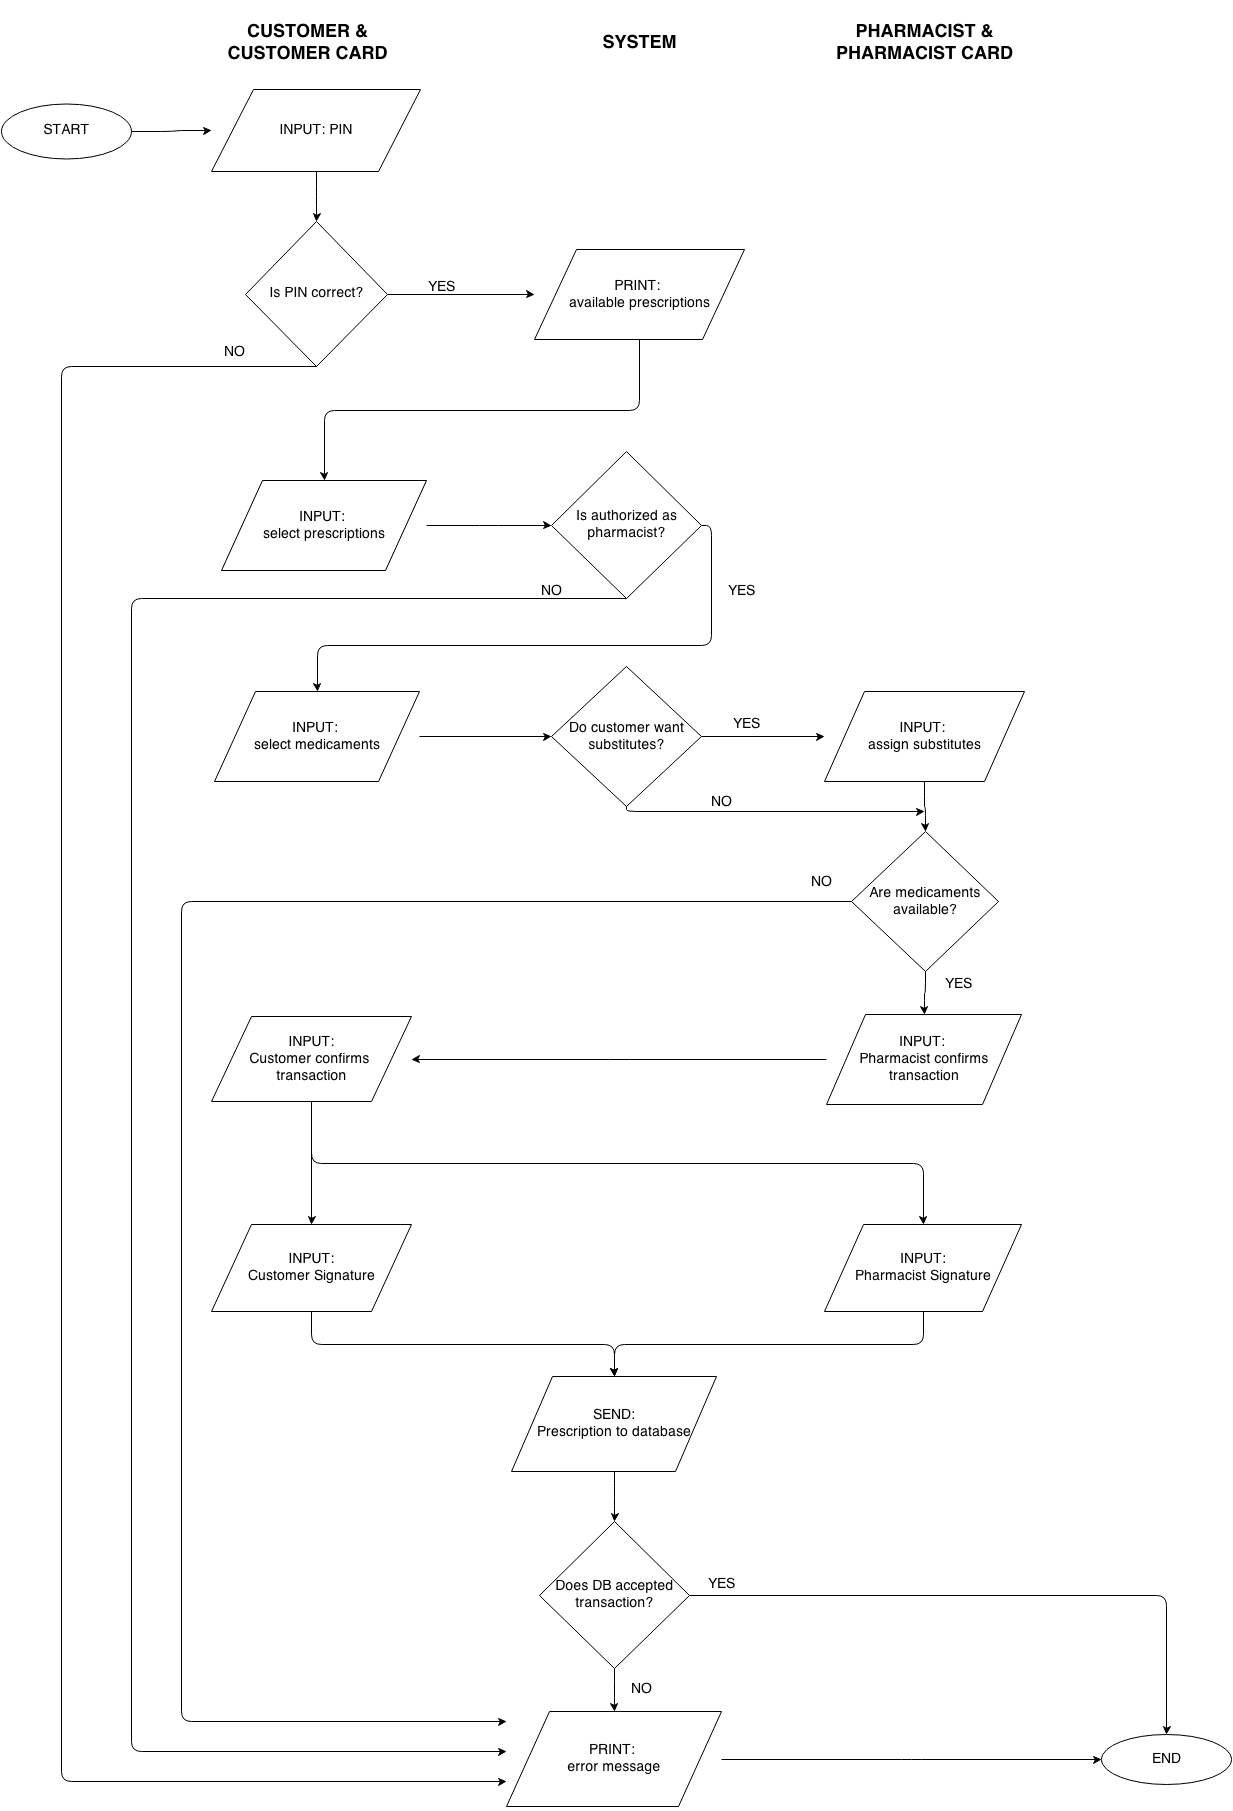
\includegraphics[width=0.98\textheight]{flow-chart.png}
    \caption{Flow chart}
    \label{fig:flowchart}
\end{figure} 

